
%
%  cognome-tesina - easy report main template
%

% TeXstudio: SET THIS FILE AS 'EXPLICIT ROOT DOCUMENT"


% --- texstudio magic comment
% ! master
% !TEX encoding = UTF-8
% !TeX program = pdflatex
%% !TeX program = xelatex
% !TeX root = "report01.tex"
% %  !TeX spellcheck = en_US
% !TeX spellcheck = it_IT

%  a4 paper, two columns italian language



\documentclass[a4paper,12pt]{report}
\usepackage{textcomp}
\usepackage{easyrep} % an agile style for report wirting
                     % see comments at the beginning of 
                     % the package file





% =============================================================================

%\input{hyphen_it.input.tex} 	% hyphenation rules

% -------------------------------------------
% cover definition
\Title{Computer vision course}
\Subtitle{Lab 6 - Image matching}
\Author{Pietrobon Andrea}
\Date{\today}



% -------------------------------------------
% local cmds
% (-- put here user defined macros--)



% -------------------------------------------
\begin{document}

\printCover       % print a cover page
%\tableofcontents  % table of contents


% -------------------------------------------
% SINGLE DOCUMENT
% nel caso di docvumenti redatti in un unico file, scrivere qui il testo

% useful text starts here

%\chapter{Intro}
%Qui il testo ... \\

%\Vispa

% -------------------------------------------
% MULTIPLE DOCUMENTS
% nel caso di documenti multipli includere qui 
% i file corrispondenti
% es.

%
%  void-input - easy report template for included file
%  EDIT THE LINE ABOVE FOR DOCUMENTATION OF THIS FILE, then delete this line! 
%         

%

% ============================================================
% --- texstudio magic comment: 
% !TEX encoding = UTF-8
% !TeX program = pdflatex
%% !TeX program = xelatex
% !TeX root = "cognome-tesina.tex"
% %  !TeX spellcheck = en_US
% !TeX spellcheck = it_IT


% ====================================================================


\chapter{Task 1}
In the first activity I had the chance to understand the behavior of the cv:cvtColor() function and I discovered that in OpenCV an RGB image is saved in a variable of type Mat in three inverted channels, such as BGR (the first blue channel, the second green and the third red). I used the COLOR BGR2GRAY parameter to transform the image into a 1 channel grayscale.

\begin{figure}[!h]
	\centering
	\begin{minipage}{1\textwidth}
		\centering
		\includegraphics[width=\linewidth]{images/source/task1/1}
		\caption{Grayscale image obtained from the original RGB.}
		\label{fig:1}
	\end{minipage}
\end{figure}

\chapter{Task 2}
The second task was slightly more complicated. I ran into some initial difficulty as the image didn't change (don't know why yet). Next, applying maxfilter (\ref{fig:2a}) and minfilter (\ref{fig:2b}) were the hardest spots. To define these functions, I had to think about how to define a kernel (filter), take a part of the whole image (with the same kernel size), calculate the maximum pixel value of all filters, and replace it with the average value in the nut. Also, one mistake that cost me a lot of time was to use the same modified image to compute subsequent kernel values. This meant that every image was ruined by the filter. Once this small but annoying problem has been fixed, we still need to figure out how to apply the filter to the last row and last column of the image. (I thought about adding rows and columns to the image, but I'm sure that's not the correct implementation).
In any case, as you can see in the image below, the maxfilter was the best filter to remove cables from the background, and the perfect kernel size not to corrupt the image too much was 5. The minfilter, however, put highlight the dark details even more.

\begin{figure}[h]
	\centering
	\begin{minipage}{0.45\textwidth}
		\centering
		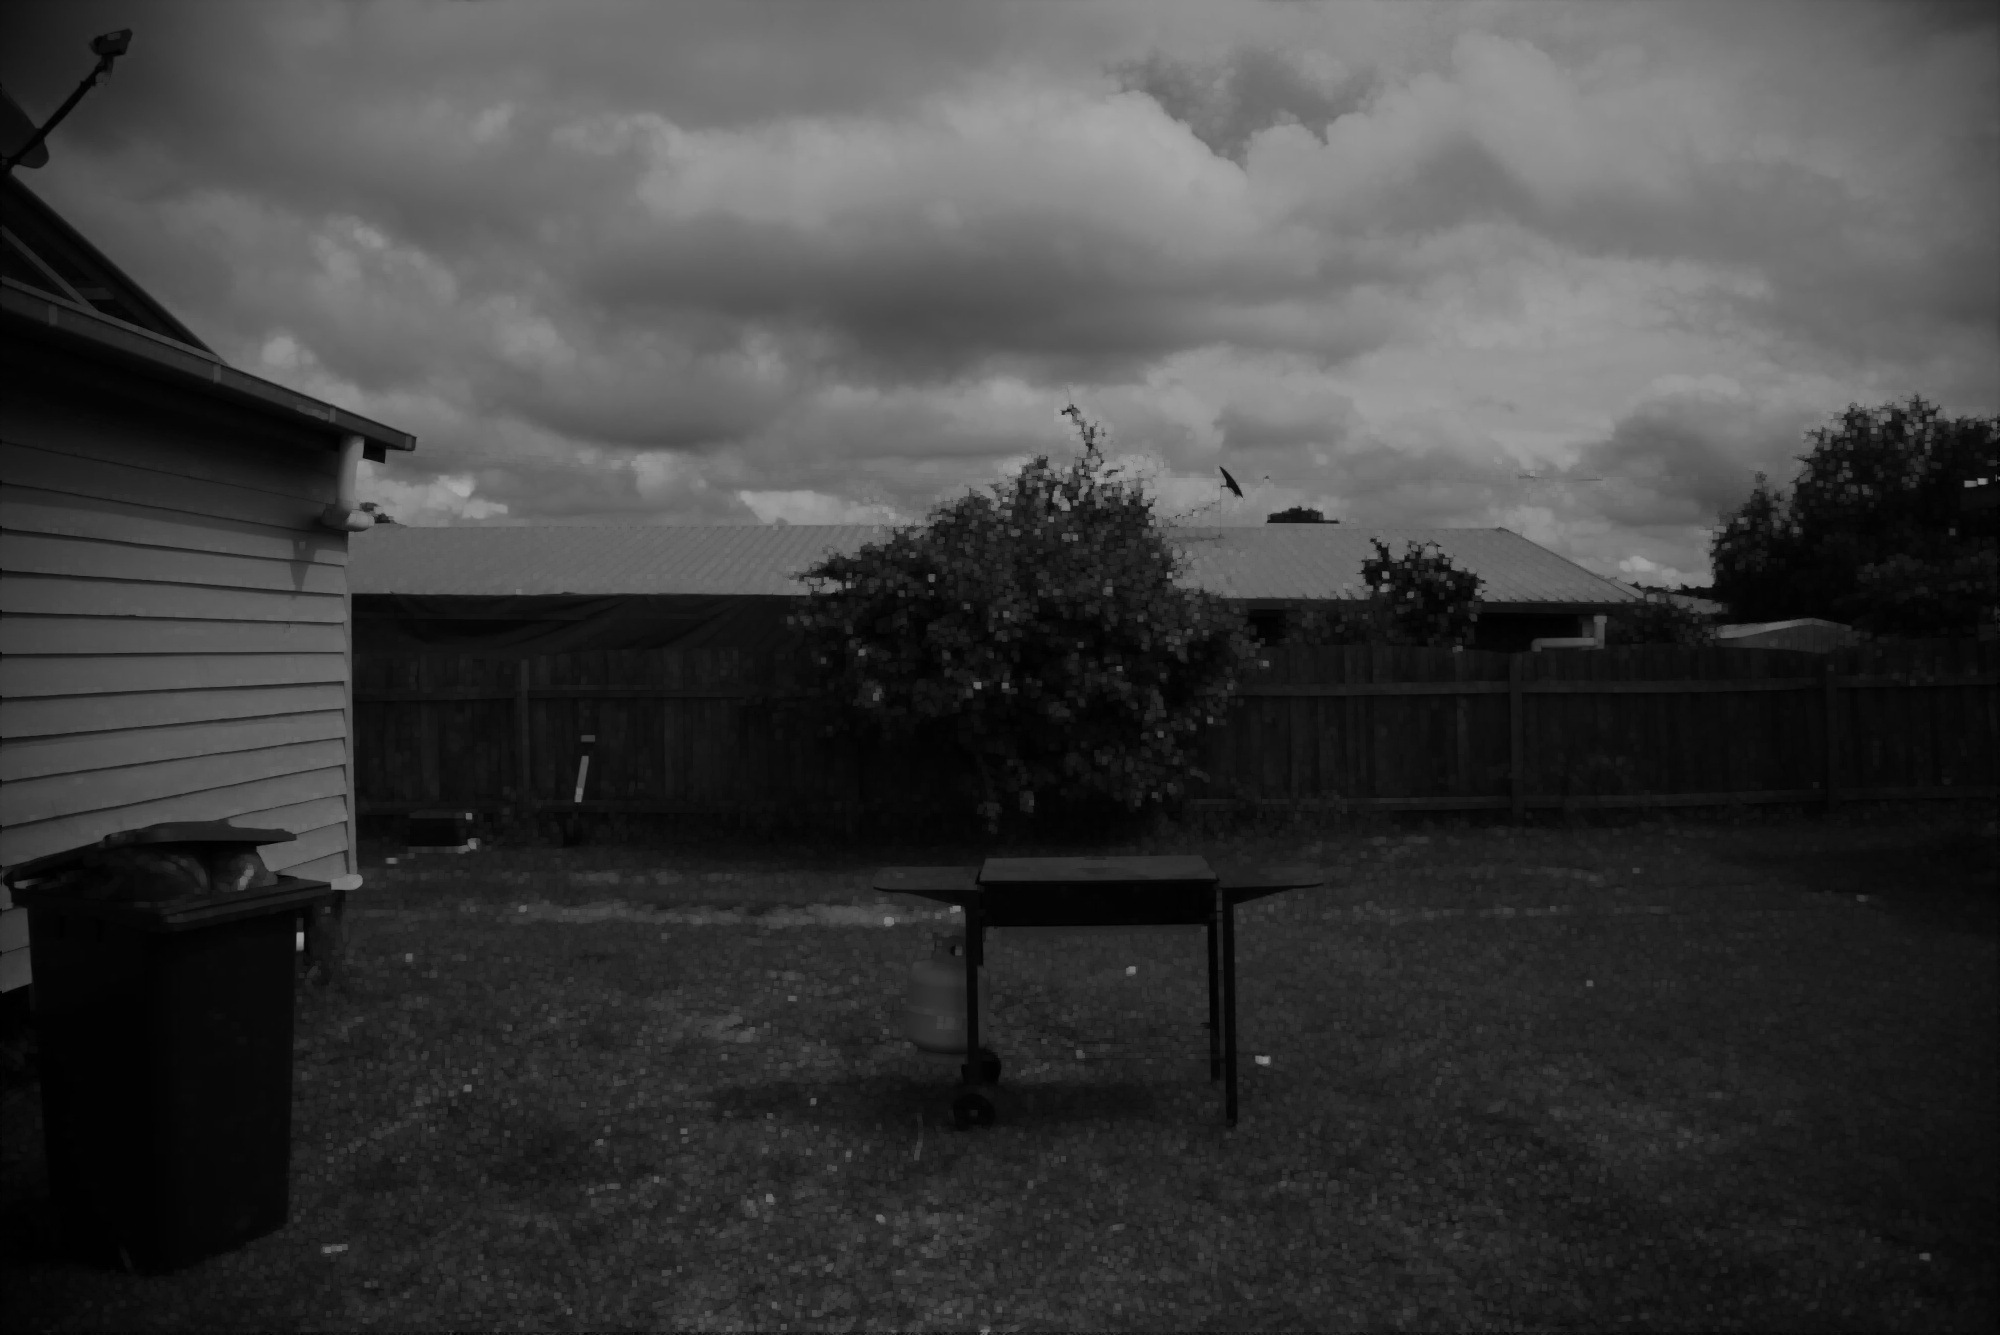
\includegraphics[width=\linewidth]{images/source/task2/1_max_5}
		\caption{Grayscale image with Max Filter and kernel size 5.}
		\label{fig:2a}
        \end{minipage}
        \hspace{0.05\textwidth}
        \begin{minipage}{0.45\textwidth}
        		\centering
		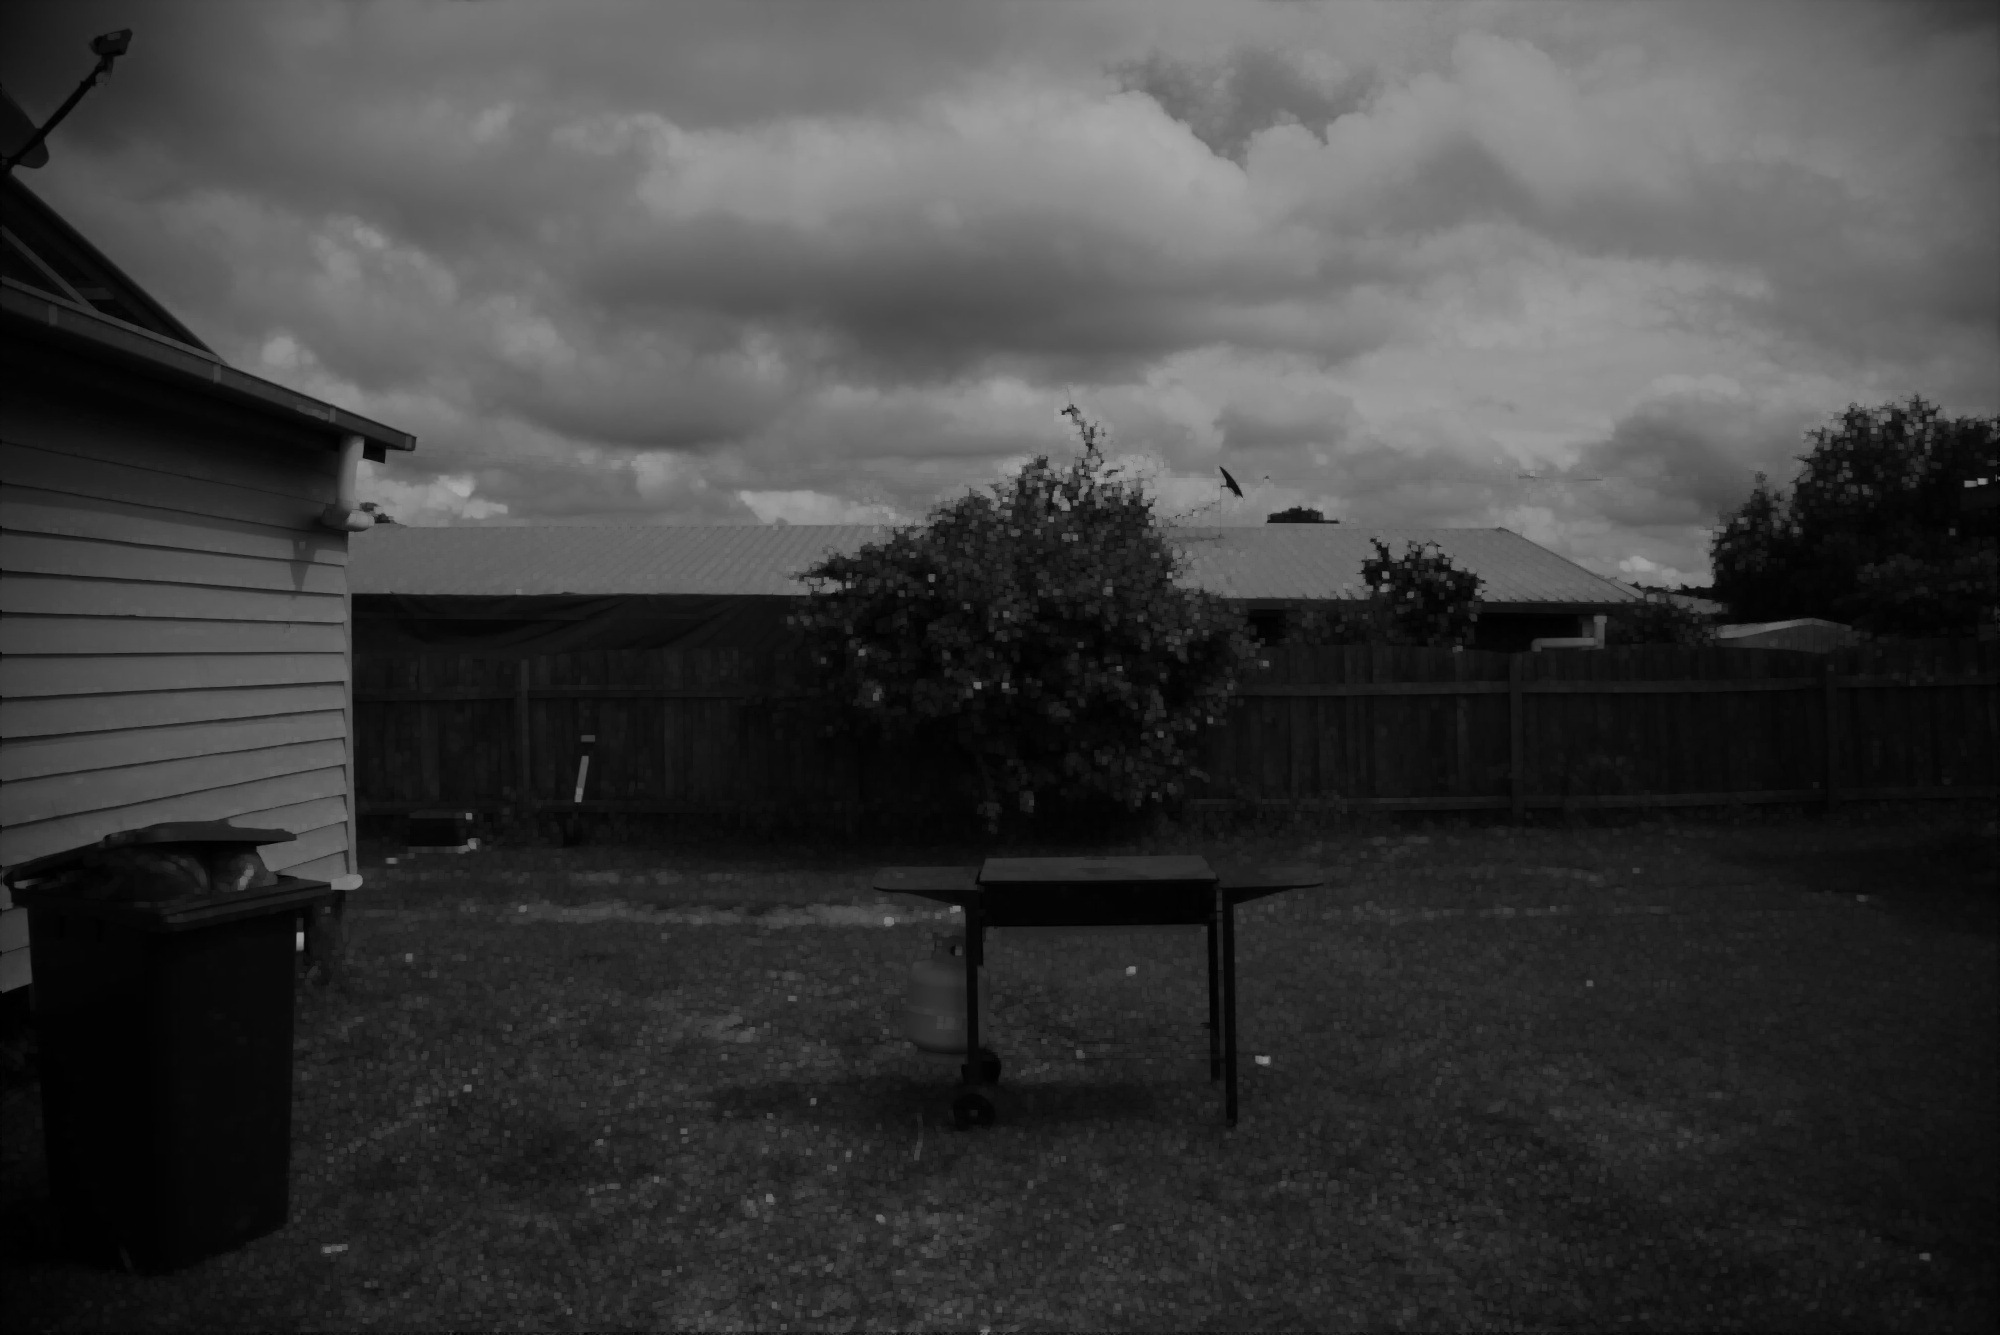
\includegraphics[width=\linewidth]{images/source/task2/1_min_5}
		\caption{Grayscale image with Min Filter and kernel size 5.}
		\label{fig:2b}
        \end{minipage}
\end{figure}

\chapter{Task 3}
Not too difficult task. I found the functions on the openCV documentation very easily and I implemented them by increasing the ksize to see the differences well as shown in  (\ref{fig:3a}) and in  (\ref{fig:3b}).

\begin{figure}[h]
	\centering
	\begin{minipage}{0.45\textwidth}
		\centering
		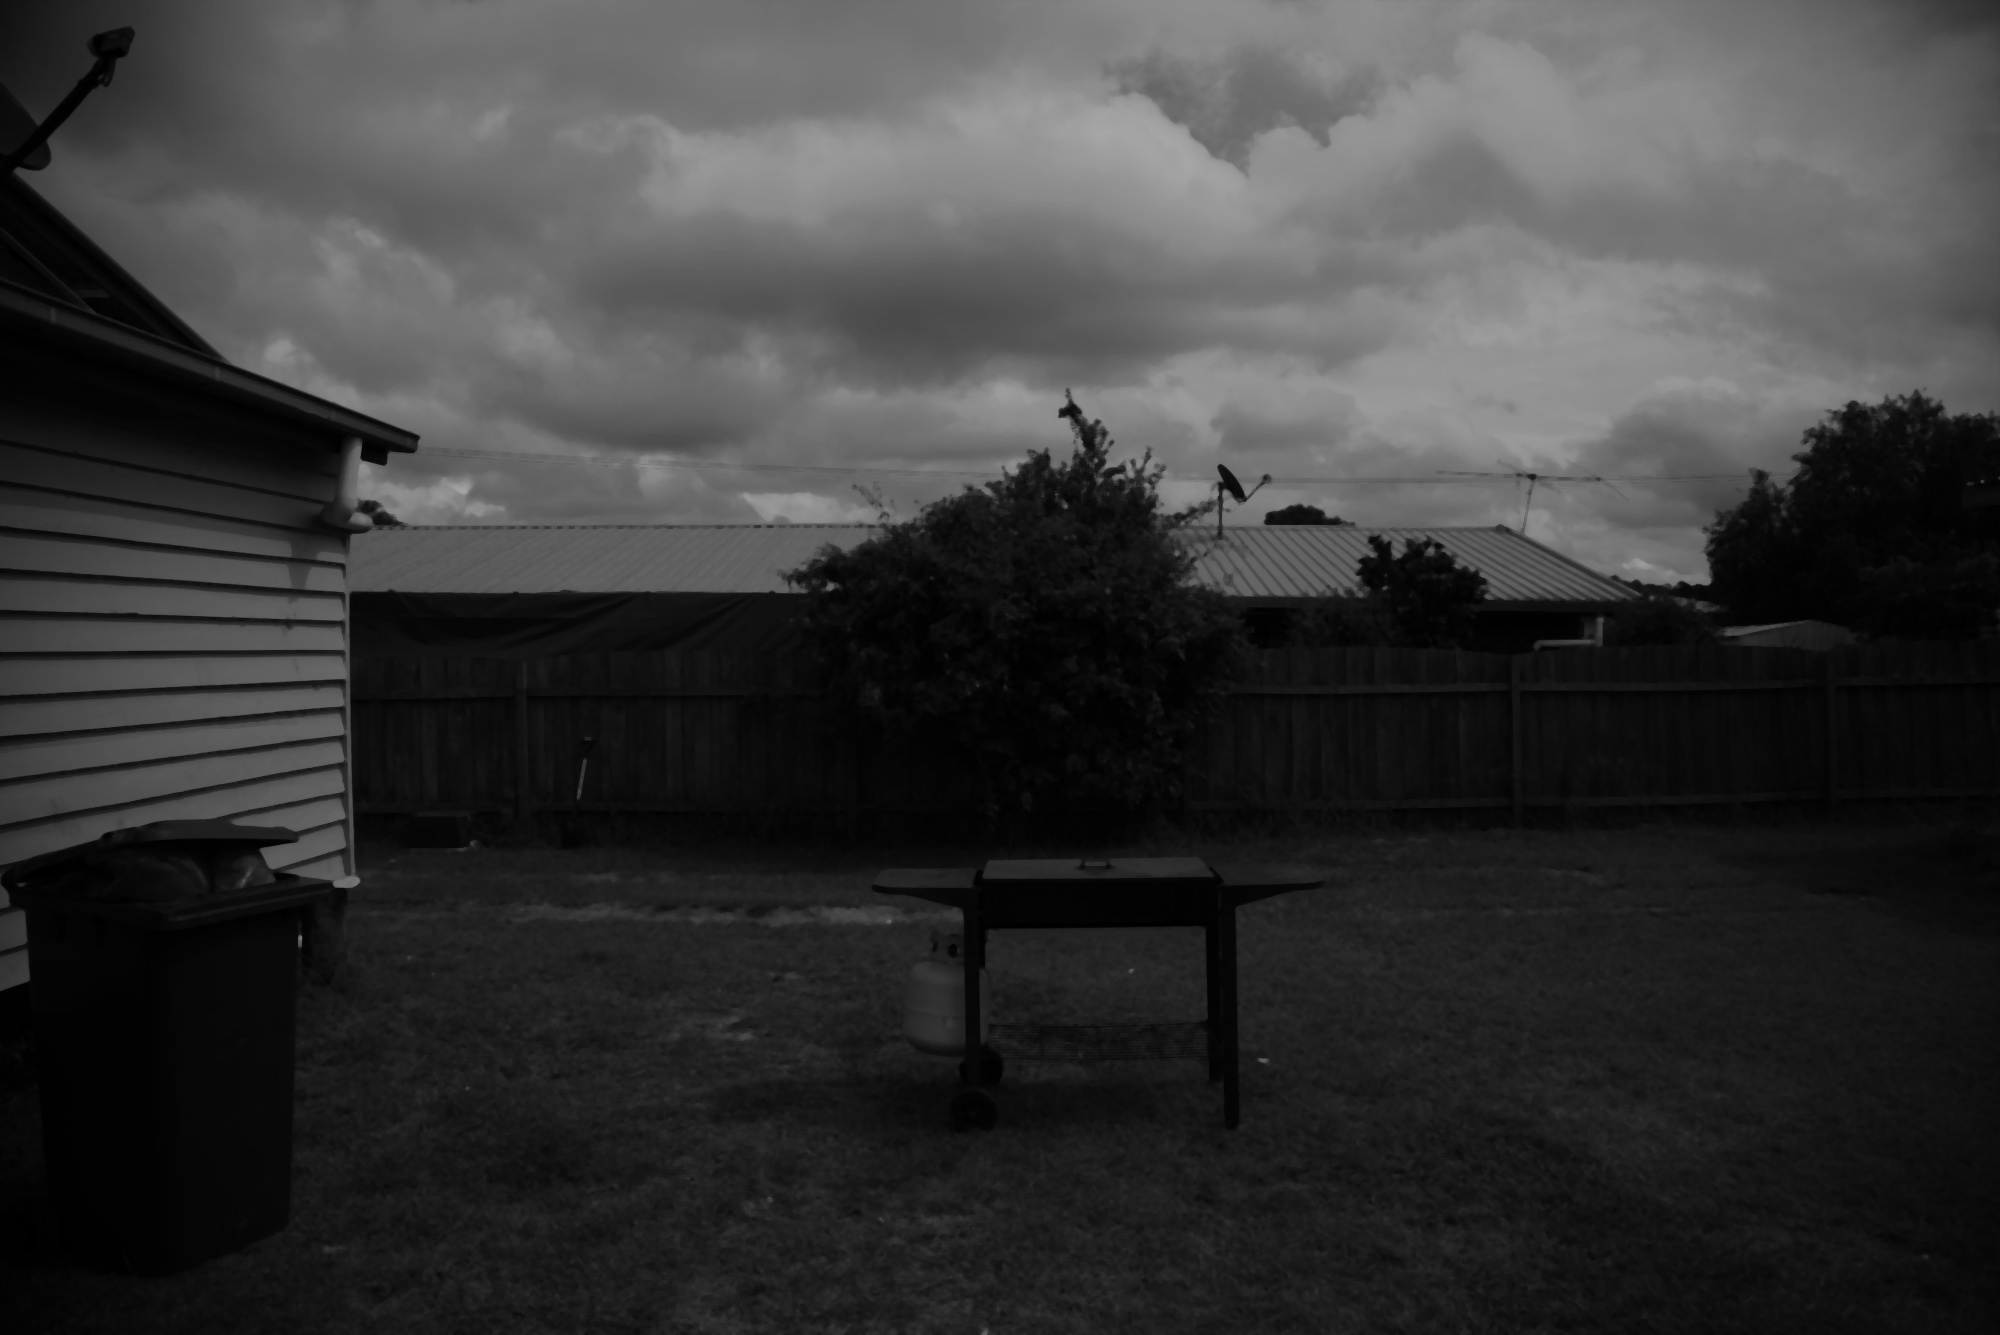
\includegraphics[width=\linewidth]{images/source/task3/median_5}
		\caption{Grayscale image with Median Filter and kernel size 15.}
		\label{fig:3a}
        \end{minipage}
        \hspace{0.05\textwidth}
        \begin{minipage}{0.45\textwidth}
        		\centering
		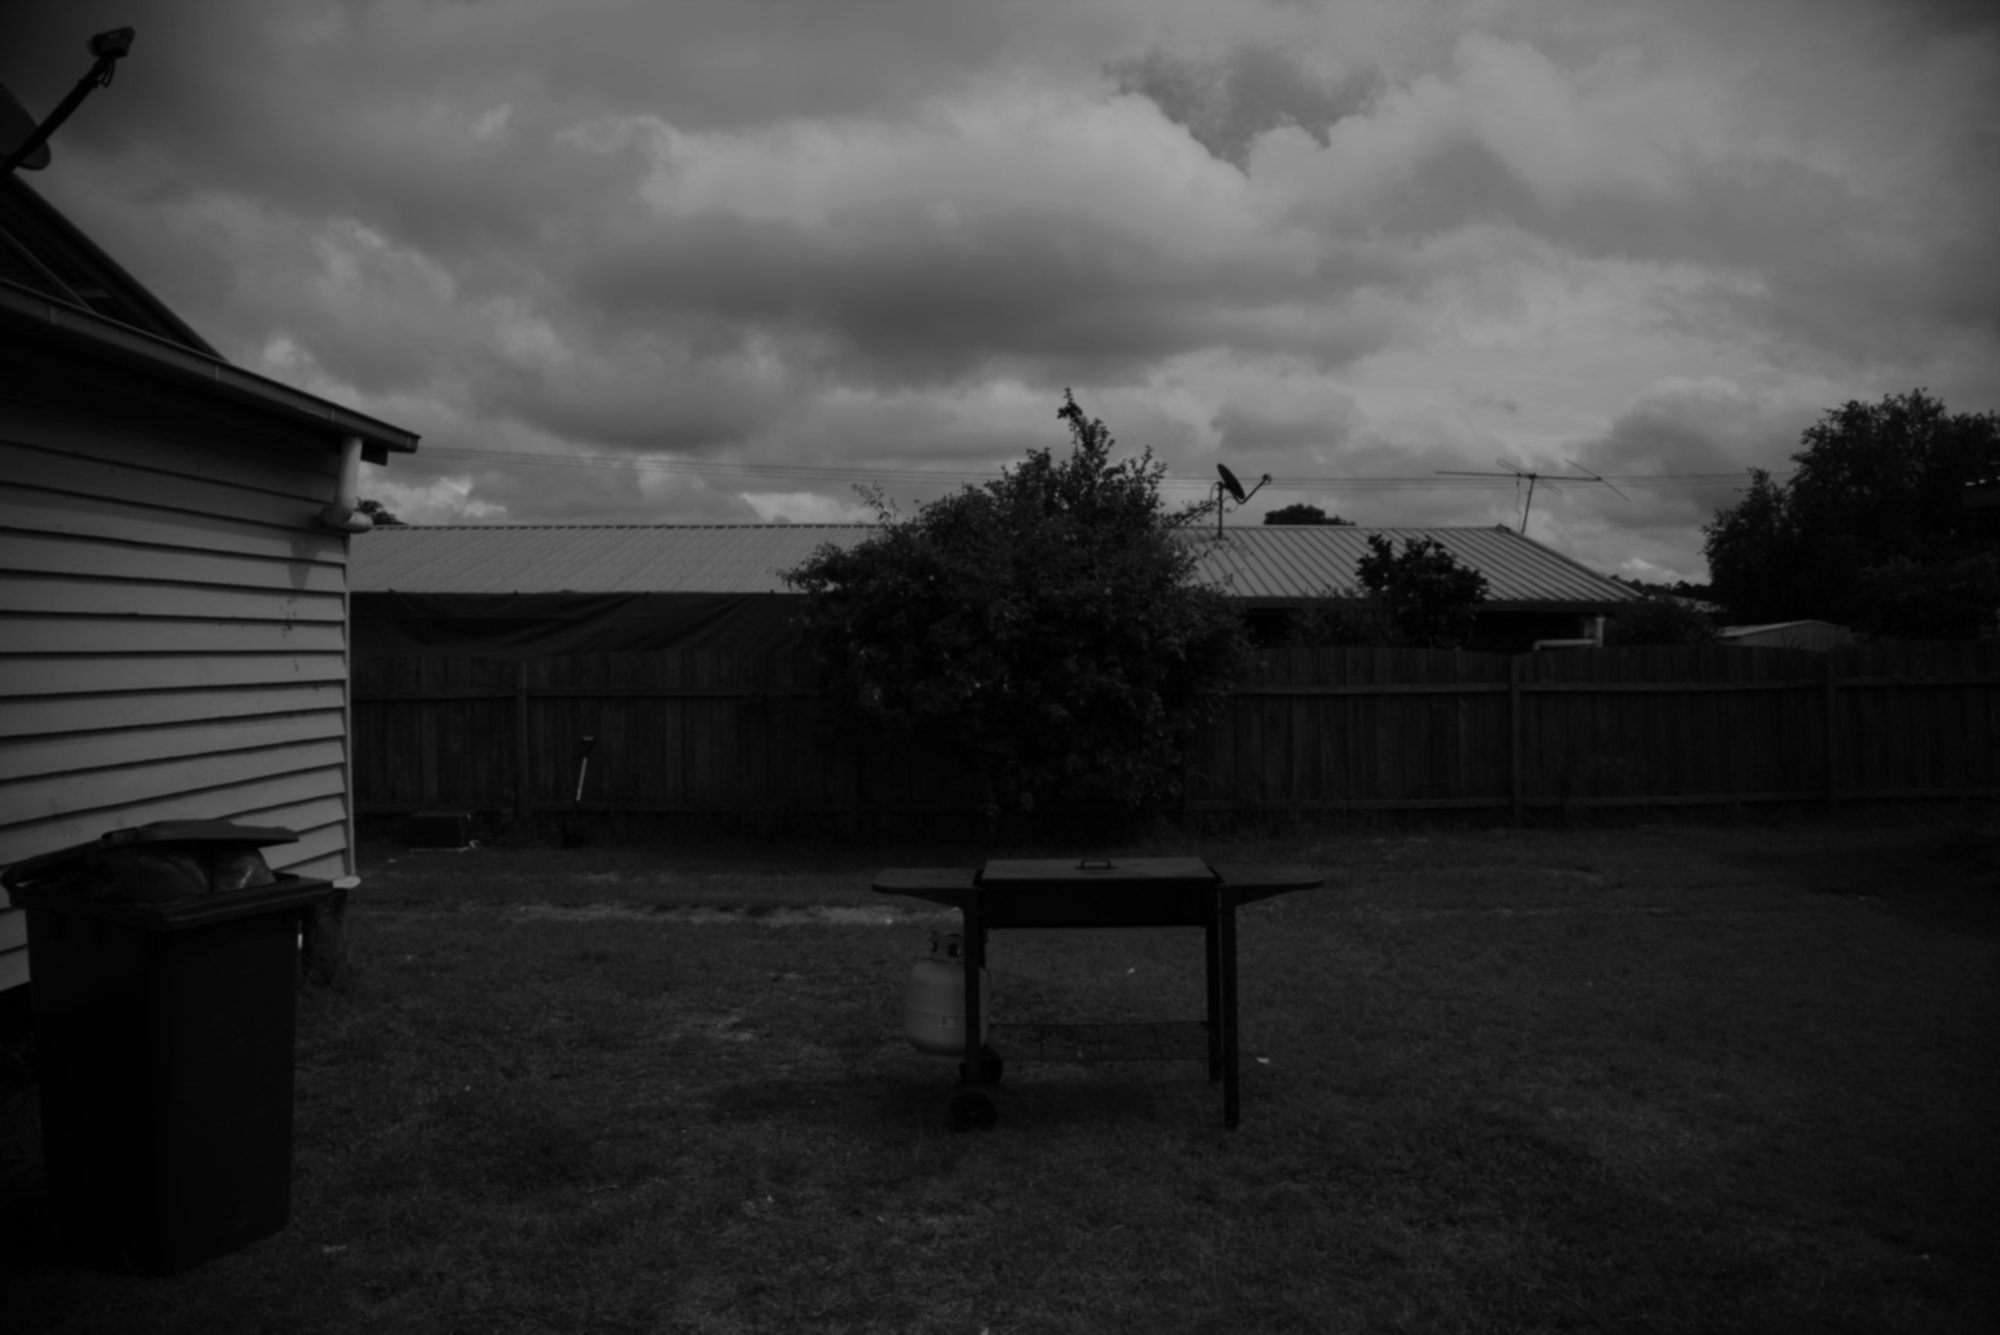
\includegraphics[width=\linewidth]{images/source/task3/gaussian_5}
		\caption{Grayscale image with Gaussian Filter and kernel size 15x15.}
		\label{fig:3b}
        \end{minipage}
\end{figure}


\chapter{Task 4}
Implementation-level simple task. Once you found an example on the offi- cial openCV documentation, you just had to apply the steps to the letter. The most ”complicated” part was actually understanding the various steps and what they were going to do to recreate the histogram. In the images below we can see the original image in the (\ref{fig:4a}) and its histogram in the(\ref{fig:4b}).

\begin{figure}[h]
	\centering
	\begin{minipage}{0.45\textwidth}
		\centering
		
\includegraphics[width=\linewidth]{images/source/task4/2}
		\caption{Original Image.}
		\label{fig:4a}
        \end{minipage}
        \hspace{0.05\textwidth}
        \begin{minipage}{0.45\textwidth}
        		\centering
		\includegraphics[width=\linewidth]{images/source/task4/1}
		\caption{Histogram of the Image with 256 bins.}
		\label{fig:4b}
        \end{minipage}
\end{figure}

\chapter{Task 5}
To complete this last task it was sufficient to use cv::equalizeHist() on the grayscale image and then slightly modify the code of task4 by removing the extra channels. I did not find any particular difficulties in carrying out this task.The equalized image and the corresponding histogram are shown below on \ref{fig:5a} and \ref{fig:5b}.

\begin{figure}[h]
	\centering
	\begin{minipage}{0.45\textwidth}
		\centering
		\includegraphics[width=\linewidth]{images/source/task5/1}
		\caption{Equalized Image.}
		\label{fig:5a}
        \end{minipage}
        \hspace{0.05\textwidth}
        \begin{minipage}{0.45\textwidth}
        		\centering
		
\includegraphics[width=\linewidth]{images/source/task5/2}
		\caption{Histogram of the Image.}
		\label{fig:5b}
        \end{minipage}
\end{figure}




% ====================================================================

% ====================================================================
% memo available commands
% ====================================================================
% easyrep: summary of provided macros
%
% \Title{text}     defines the document title 
% \Subtitle{text}  defines the subtitle
% \Author{text}    defines the author string
% \Date{text}      defines a date string
% \printCover      print a cover page using above information
%
% --- text styles
% \tDef{text}      definition (generic) 
% \tDefObj{text}   definition (the ter being defined)
% \tDefTxt{text}   definition (the statement defining the term) 
% \tRemark{text}   remarked text
% \tREMARK{text}   highly remarked text 
% \tLoud{text}     shouted text! 
% \tCode{text}     inline code text
% \tLatin{text}    latin text
% \tForeign{text}  foreign language text 
% \tExample{text}  example 
% \tStandard{text} a recommendation 
% \tQuote{text}    a quoted text 
% \tQuoteFig{text} a quoted text referring to a figure 
% \tConcept{text}  an important concept  
% \tBeginPar{text} highlighted text 
%                  at the beginning of a paragraph 
%
% ---environments
% \begin{quoteStandard} text... \end{quoteStandard}
%    print text to be quoted, e.g. sentences from 
%    a recommendation
%
% \begin{quoteRemark} text... \end{quoteRemark}
%    similar to quoteStandrd, but the text is more marked
%
%  
% --- typo accelerators
% \qmo             opening quotation mark (use \qmo{})
% \qmc             closing quotation mark (use \qmc{})
% \th  emphasises "th"
% \ie  slanted "i.e."
% \eg  slanted "e.g."
% \es  slanteg "ad es."
% \octave   "octave" in \tCode style
% \matlab   "matlab"
% \labview  "labVIEW"
% \latex    "LaTeX" (just the text!)
%
% --- math typo accelerators
% \v{math text}  underlines the math text (useful for vector) 
%
% --- debug commands
% \debugTextStyles        print a table showing text styles
% \debugPrintCharacters   print a table of characters
% \Vispa                  print some text (to fill)  
% \Vispas                 more filling text
% ====================================================================
 
%\input{void-input.tex} 



% ------------------------------------------------------
% bibliography
% - comment \cite{*} if you want toinclude references that are explicitly 
%   quoted in the preceding text
% - add/modify bibtex files in the \bibliografy command 
\clearpage
%\addcontentsline{toc}{chapter}{Bibliography}
%\nocite{*} % inserts ALL the references contained in the
           % ".bib" files defined by the  following "\bibliography{}" commands
%\bibliography{bib/bib-iq,bib/bib-stat,bib/bib-iq-web.bib}
%\bibliography{bib/bib-pietrobon_report}
%\bibliographystyle{ieeetr} % acm siam abbrv plain, alpha, abbrv, ieeetr


% ------------------------------------------------------




% ====================================================================
\end{document}
% ====================================================================



% ====================================================================
% ====================================================================




% ====================================================================
% memo available commands
% ====================================================================
% easyrep: summary of provided macros
%
% \Title{text}     defines the document title 
% \Subtitle{text}  defines the subtitle
% \Author{text}    defines the author string
% \Date{text}      defines a date string
% \printCover      print a cover page using above information
%
% --- text styles
% \tDef{text}      definition (generic) 
% \tDefObj{text}   definition (the ter being defined)
% \tDefTxt{text}   definition (the statement defining the term) 
% \tRemark{text}   remarked text
% \tREMARK{text}   highly remarked text 
% \tLoud{text}     shouted text! 
% \tCode{text}     inline code text
% \tLatin{text}    latin text
% \tForeign{text}  foreign language text 
% \tExample{text}  example 
% \tStandard{text} a recommendation 
% \tQuote{text}    a quoted text 
% \tQuoteFig{text} a quoted text referring to a figure 
% \tConcept{text}  an important concept  
% \tBeginPar{text} highlighted text 
%                  at the beginning of a paragraph 
%
% ---environments
% \begin{quoteStandard} text... \end{quoteStandard}
%    print text to be quoted, e.g. sentences from 
%    a recommendation
%
% \begin{quoteRemark} text... \end{quoteRemark}
%    similar to quoteStandrd, but the text is more marked
%
%  
% --- typo accelerators
% \qmo             opening quotation mark (use \qmo{})
% \qmc             closing quotation mark (use \qmc{})
% \th  emphasises "th"
% \ie  slanted "i.e."
% \eg  slanted "e.g."
% \es  slanteg "ad es."
% \octave   "octave" in \tCode style
% \matlab   "matlab"
% \labview  "labVIEW"
% \latex    "LaTeX" (just the text!)
%
% --- math typo accelerators
% \v{math text}  underlines the math text (useful for vector) 
%
% --- debug commands
% \debugTextStyles        print a table showing text styles
% \debugPrintCharacters   print a table of characters
% \Vispa                  print some text (to fill)  
% \Vispas                 more filling text
% ====================================================================
